This introductory chapter describes some general information you
need to know about how to perform laboratory procedures, how to write a 
lab worksheet and how to
analyze data correctly. Please read these through carefully; your instructor 
will cover these items quickly on the first day of lab, and you should already
be familiar with these ideas before you come to class.

\section{General Lab Procedures}

Physics 103N is a three hour lab designed to be self-contained.
This means that your only homework is to prepare for the next lab.
You {\it must} do this preparation.  
The type of laboratory report you will submit at
the end of the class period is a worksheet lab.  You will fill
out a worksheet as you proceed through the experiment.
You will spend
two hours in lab collecting data and plotting graphs.  At the end of the
second hour, you will move to a classroom and complete your calculations
and discussions for that day's lab and turn in the finished worksheet
to your instructor.    If you are unprepared and unable
to complete the worksheet, you must hand it in by the end of the third hour
anyway.
We designed this format to help you 
focus on the physical meaning of the experiments and avoid sinking into a 
morass of meaningless calculations. 

To help you avoid many hours of tedious number crunching, we have placed 
computers in the lab. You should use these to do most, if not all, of your 
graphing and major numerical manipulations. However, the computer cannot think
for you; you have to assess whether the computer is handing you garbage or if 
the results are reliable. Here are some things to keep in mind about the 
computer
\begin{itemize}
\item  It cannot keep track of units.
\item  It must be taught how to deal with uncertainties.
\item  It will not automatically place error bars on your graphs.
\end{itemize}

You must complete the worksheet by the end of class; therefore, your 
instructor may deem a quiz unnecessary, since you must be prepared to complete
the worksheet on time.  The possibility of a quiz exists, however, so know
the rudiments of the procedure of the day. To prepare, you should read the 
manual over very carefully before you come to class. This means you should 
understand the lab goals and important equations.


\section{Error Estimation and Propagation}

Error is everywhere, and you must not only acknowledge it, but understand it 
and control it. Webster defines ``error'' as the ``difference between 
an observed or calculated value and the true value.'' The problem with this 
definition is that we usually have no idea what the ``true'' answer should be.
Previous experiments or theoretical calculations may give us a clue, but 
somehow we must extract an estimate of the true value from our data. In 
addition, we should also determine to what extent we should take our answer 
seriously. This last point embodies what we call error estimation. 

An example will show why this process is so important. Suppose you measure the
acceleration of a free-falling body and the answer you obtain is $10.5~{\rm
 m/s^2}$. Have you contradicted the accepted value of $9.7990 \pm 0.0014~{\rm
 m/s^2}$? The answer depends on the size of the error in your answer. If your 
result was $10.5 \pm 1.0~{\rm m/s^2}$ then your answer is no, because the 
accepted value lies within your error. If, on the other hand, you had 
performed a fairly precise measurement and obtained $10.5 \pm 0.1~{\rm 
m/s^2}$, then your answer would have to be yes; you should then start looking 
for what went wrong in the experiment itself, since many, many other 
measurements conducted over the last 300 years have established the accepted 
value $9.7990 \pm 0.0014~{\rm m/s^2}$. So, the amount of effort and trust you 
put into an answer depends critically on ascertaining the correct overall 
uncertainty.

Rarely is what you measure directly comparable to other experimental results 
or theoretical calculations; typically, you must process your data through 
various formulas to extract a parameter you can compare with others. 
Therefore, it is critically important to accurately {\em propagate} the 
uncertainties in the original data through the calculations and arrive at a 
reasonable uncertainty for the final value. This is the process of error 
propagation. These are the issues that we now discuss.

\subsection{Definition of Uncertainty}

The first step involved in error estimation is to identify the possible types 
of errors that can occur in your experiment. There are three basic types you 
need to be aware of: illegitimate errors, systematic errors, and random errors. 
Illegitimate errors are faults in experimental procedures or 
calculational blunders. We will make every effort to avoid making these kinds 
of errors, but if we do blunder, we can easily find and correct
them; {\em we will assume that we have eliminated all illegitimate errors 
from our experiments.} This is a formidable assumption since the time to 
perform our experiments is limited; however, the procedures are not all that 
complicated; so this assumption should not be a bad one. Under this assumption
therefore, we cannot use illegitimate errors as reasonable explanations for
any discrepancies that ultimately occur in our analysis. To discuss the other
types of errors, we must more carefully distinguish between accuracy and 
precision.

{\em Accuracy} represents how close a measurement is to the true value. 
{\em Precision} indicates how well the results of an experiment have been 
determined, independently of how well the results agree with the true value.
This tells us about the self-consistency of a measurement. When judging the 
results of an experiment, we must consider both the accuracy and the 
precision. In general, when we quote the uncertainty of an experimental 
result, we are referring to the {\em precision} with which the result has been 
determined.

{\em Systematic errors} are errors that make our results different from  the 
true value in a reproducible way. They are usually due to the faulty 
calibration of equipment or some unknown bias on the part of the experimenter. 
They can be subtle and hard to quantify. Knowledge of the apparatus and the 
experimental procedure is the central manner of minimizing the impact of 
systematic errors in our results. Such errors affect the {\em accuracy} of our 
results, since  they contribute the same amount of discrepancy each time we 
perform the experiment. {\em Random errors}, on the other hand, constitute the 
major source of imprecision in an experiment. These are the random 
fluctuations in measurements from experiment to experiment, primarily due to 
the finite resolution of our apparatus. To control random errors, we must 
perform the experiment many times and use a statistical analysis to extract 
our results. A given accuracy implies at  least an equivalent precision; thus, 
accuracy depends on these fluctuations too.

To clarify the difference between these two types of errors, consider the
simple experiment of determining the average speed of a rolling ball as it
passes by a meter stick, by using a handheld timer. A systematic error
involved in this experiment could be due to the calibration of our instruments.
For instance, assume that the intervals on the meter stick are 1\% larger than
they should. Then, every time we record a distance of 50~cm the actual distance
travelled by the ball is 50.5~cm. The distinct feature of systematic errors,
such as this, is their repeatability. No matter how many times we perform the
same measurement, if we are using the same instrument, we will always make the
same ``mistake.'' Random errors don't share this property. In the rolling ball
experiment a random error is due to the timer operator. No matter how hard he
or she tries, a human operator cannot be entirely consistent on when to press
the start/stop button on the timer. Sometimes, he or she will start the timer
just a little before the ball passes by the predetermined mark on the ruler,
some times a little after. The same thing will happen when it is time to stop
the timer. The end result is that, if we perform many attempts at the
experiment (and assuming that the ball is always launched at the same speed,)
the times we will get will vary randomly around the correct value. A random
error is also introduced by the finite resolution of the devices we are using.
Suppose that we have replaced the timer's human operator with a ``perfect''
photogate setup. If the smallest time increment on our timer is 0.01~s and we
measure a time of 50.23~s then we only know that the actual time is between
50.225~s and 50.235~s. Every value in between these two will be rounded and
displayed on our instrument as 50.23~s. If we perform the measurement many
times and we always get the same reading of 50.23~s, the reasonable thing to
assume is that, in every attempt, the actual time was different, but
within the above-mentioned limits.

We also distinguish between what we call absolute and relative uncertainty.
{\it Absolute uncertainty} is the uncertainty in a quantity expressed in the 
same units as the quantity. For example, if we write
$$ g = 9.7990\pm 0.0014~\mbox{m/s}^2,$$ 
then the absolute uncertainty in the measurement of $g$ is 
$\Delta g=0.0014~\mbox{m/s}^2$.  Note that we always consider the absolute 
uncertainty to be a {\it positive} number. The {\it relative uncertainty} is 
the uncertainty expressed as a fraction or percentage of the quantity.  The 
relative uncertainty of $g$ in our example is 
$$ \frac{\Delta g}{g} = \frac{0.0014~\mbox{m/s}^2}{9.7990~\mbox{m/s}^2}
= 0.00014 = 0.014\%.$$ 

\subsection{Estimating Quantities and Their Uncertainties}
\label{sec:intro:uncert}
Now that we know what constitutes error, we should describe how to estimate 
it given a data set. Let's consider the most common situation in which we 
need to extract an estimate for the error; this occurs when we've made several
measurements of the same quantity and we want to extract an average value and 
a corresponding uncertainty. For concreteness, suppose we have a set of $N$ 
data points $x_i$ with uncertainty $\Delta x_i$ which we do not assume is the 
same for each of the measurements. (We need this generality because the 
uncertainty can vary independently of  the quantity being measured; for 
example, if you measure a current value on two different scales on a meter, 
then the uncertainties of the two measurements are different.) Then you can 
show ({\it c.f.}~Bevington and Robinson, see the Preface for the reference) 
that, assuming a Gaussian error distribution, the {\bf most probable value} is the 
mean, or average, value, $\overline{x}$:
\begin{equation}
\fbox{$ \displaystyle \overline{x} = \frac{\sum^{N}_{i=1} \frac{x_i}{(\Delta x_i)^2}}
{ \sum^{N}_{i=1} \frac{1}{(\Delta x_i)^2}}. $}   \label{eq:intro:average}
\end{equation}
This formula may look complicated, but all it does is give prominence to those 
measurements with the smallest uncertainty, a very reasonable thing to do. 
Notice that, if all the values have the same uncertainty, $\Delta x_i = \Delta 
x$ for $i=1$ to $N$, this formula reduces to the usual $\overline{x} = (1/N) 
\sum^{N}_{i=1} x_i$.   The corresponding uncertainty in the average value is 
the {\bf standard deviation}, $\sigma$, and comes from  the relation
\begin{equation}
\fbox{$ \displaystyle \frac{1}{\sigma^2} = \sum_{i=1}^{N} \frac{1}{(\Delta x_i)^2}. $}
\label{eq:intro:standdev}
\end{equation}
We can see from this formula that the uncertainty of  the combination is 
always less than the smallest uncertainty of the component measurements. We 
should certainly hope so! After all, the more measurements we do, the better 
we should know what the answer is. In the case that all the uncertainties are 
equal to $\Delta x$, this expression reduces to $\sigma = \Delta x / 
\sqrt{N}$, showing that the uncertainty decreases at the relatively slow rate 
of one over the square root of the number of measurements.

Suppose you have three measurements of the resistance of a resistor that have 
come from three different techniques. This data appears in 
Table~\ref{tab:intro:resistance measurements}. The nominal value is the value 
printed on the resistor; the multimeter measurement comes from an ohmmeter 
measurement; and the current and voltage measurements come from a detailed 
analysis using Ohm's law. Each technique has its own associated uncertainty. 
We want to combine these separate measurements into a single estimate of the 
resistance. Since the errors are distributed symmetrically ({\it i.e.}, 
another measurement's value is equally likely to fall on either side of the 
current measurement's value), we can reliably use our formulas based on a 
Gaussian distribution, {\it i.e.}, the ones given above. We find the 
resistance to be
\begin{eqnarray*}
2.5866 \pm 0.0027~{\rm k} \Omega.
\end{eqnarray*}
This answer reflects several general features of these formulas mentioned 
above. First, it is closest to the measurement with the smallest uncertainty. 
Second, the uncertainty of  the combined measurements is less than the 
smallest measured uncertainty, but not by much. This reflects the fact that 
the other measurements' uncertainties were much larger than the last. This is 
good intuition that you should incorporate into your thinking patterns; it 
will help you identify the important sources of error in your experiments.
\begin{table}[htb]
\begin{center}
\begin{tabular}{l|c}
Experimental Technique & Value\\
\hline
Nominal Value & 2.70 $\pm$ 0.14 k$\Omega$\\
Multimeter        & 2.69 $\pm$ 0.01 k$\Omega$\\
Current and Voltage Measurements & 2.5785 $\pm$ 0.0028 k$\Omega$\\
\end{tabular}
\end{center}
\caption{Resistance values for a single resistor from different measurements.}
\label{tab:intro:resistance measurements}
\end{table}

For more sophisticated experiments, we don't necessarily measure the same 
quantity over and over. We might change one parameter and measure another, to 
investigate the effects of one on the other. When we do this, we are looking 
for correlations between the different parameters. One of the most effective 
ways to spot correlations is to graph the parameters and look for some 
functional relationship. The easiest and most reliable functional relationship 
to recognize and quantify is a linear one, {\it i.e.}, when you plot the 
parameters, the data points fall along a line. In fact, this type of 
correlation is so important that we sometimes alter the parameters that we 
plot to force the graphed data into a line, as in a log-log plot or a semi-log 
plot. Here, we don't just plot the data, but certain functions of the data 
that are linearly related. This can't always be done, but for our labs it can; 
so, we will focus solely on analyzing linear correlations. In this case, the 
correlation between the two quantities is described in terms of two numbers: 
the slope of the line and its $y$-intercept. For most purposes, the slope is 
the more important of the two, but the intercept can also contain important 
physical information. Once the data suggests a linear relationship, we want to 
extract the slope and intercept of the ``best fit'' line.

There are many complicated definitions of  ``best fit'' that one can use to 
extract a consistent slope and intercept from a set of data. The most often 
used method goes by the name of {\em least squares} fit. The reason for the 
popularity of this particular method has to do with its relative simplicity 
and statistical significance. It will provide the slope and intercept of the 
most probable line to fit a set of data, assuming a Gaussian distribution for 
the errors. Thus you can think of this as analogous to extracting the average 
quantity for a larger class of measurements.

We can derive the formulas for the linear least squares fit to a set of data 
with the following assumptions: first, that the uncertainty is symmetrically 
distributed about the data values, and second, the uncertainty in the 
dependent variable is more significant than the uncertainty in the independent 
variable. These assumptions are discussed at length in Bevington and Robinson, 
and we will simply take them for granted. With these assumptions in mind, we 
can proceed as follows: given $N$ data points 
$(x_i,y_i \pm \Delta y_i), i=1,\ldots,N$, we want to determine the parameters 
of the line $y=ax+b$ so that the square of the vertical distance between the 
$y$~coordinates of the line and the data, weighted by the uncertainty 
$\Delta y_i$ and summed over all the data points, is a minimum. The geometry 
of this construction is shown in Figure~\ref{fig:intro:least squares}. That is,
we want to minimize the function of 2~variables
\begin{eqnarray*}
e(a,b) = \sum^{N}_{i=1} \left( \frac{1}{\Delta y_i} (y_i-ax_i-b)\right)^2
\end{eqnarray*}
\begin{figure}[!htb]
\centering
\epsfxsize=12cm 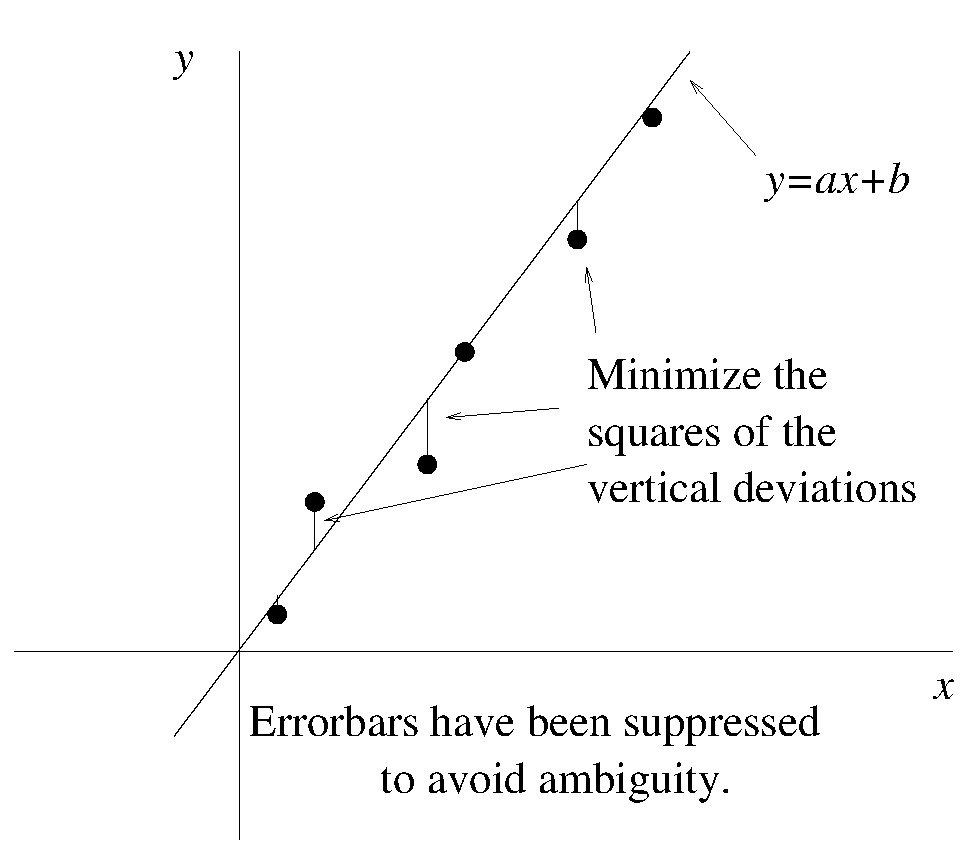
\includegraphics[scale=0.6]{0_intro/graph.eps}
%\centerline{\epsfxsize=12cm \epsfbox{intro_2/graph.eps}}
\caption{The least squares method determines the line that minimizes the 
square of the vertical distances between the line and the data.}
\label{fig:intro:least squares}
\end{figure}
To minimize this function, we take the partial derivatives with respect to $a$ 
and $b$ and set them equal to zero. This yields the following system of linear 
equations for $a$ and $b$:
\begin{eqnarray*}
a \sum^{N}_{i=1} \frac{x_i^2}{(\Delta y_i)^2} + b \sum^{N}_{i=1} \frac{x_i}
{(\Delta y_i)^2}
& = & \sum^{N}_{i=1} \frac{x_i y_i}{(\Delta y_i)^2} \\
a \sum^{N}_{i=1} \frac{x_i}{(\Delta y_i)^2} + b \sum^{N}_{i=1} \frac{1}
{(\Delta y_i)^2} & = & \sum^{N}_{i=1} \frac{y_i}{(\Delta y_i)^2} 
\end{eqnarray*}
Using your favorite technique, you can show that the solution of this linear 
system of equations is
\begin{eqnarray}
a &=&  \frac{1}{D} \left[ 
       \left( \sum^{N}_{i=1} \frac{1}{(\Delta y_i)^2}\right) 
       \left( \sum^{N}_{i=1} \frac{x_i y_i}{(\Delta y_i)^2} \right) -
       \left( \sum^{N}_{i=1} \frac{x_i}{(\Delta y_i)^2} \right)               
       \left( \sum^{N}_{i=1} \frac{y_i}{(\Delta y_i)^2} \right) \right],
\nonumber \\
b &=&  \frac{1}{D}  \left[ 
       \left( \sum^{N}_{i=1} \frac{x_i^2}{(\Delta y_i)^2} \right)
       \left( \sum^{N}_{i=1} \frac{y_i}{(\Delta y_i)^2} \right) -
       \left( \sum^{N}_{i=1} \frac{x_i}{(\Delta y_i)^2} \right)
       \left( \sum^{N}_{i=1} \frac{x_i y_i}{(\Delta y_i)^2} \right) \right],
\end{eqnarray}
where
\begin{equation}
D = \left( \sum^{N}_{i=1} \frac{1}{(\Delta y_i)^2} \right)
         \left( \sum^{N}_{i=1} \frac{x_i^2}{(\Delta y_i)^2} \right) -
         \left( \sum^{N}_{i=1} \frac{x_i}{(\Delta y_i)^2} \right)^2.
\end{equation}
The corresponding uncertainties in the fit parameters are
\begin{eqnarray}
(\Delta a)^2 &=& \frac{1}{D} \sum^{N}_{i=1} \frac{1}{(\Delta y_i)^2},
\nonumber \\
(\Delta b)^2 &=& \frac{1}{D} \sum^{N}_{i=1} \frac{x_i^2}{(\Delta y_i)^2}.
\end{eqnarray}

Let's take a look at these equations in action. Consider the data given in 
Table~\ref{tab:intro:current voltage data}; this data came from current and 
voltage measurements across a resistor of unknown resistance. Ohm's law 
indicates that, for most resistors, the voltage is linearly related to the 
current, the proportionality constant being the resistance. We've plotted this 
data in Figure~\ref{fig:intro:current voltage plot}, which strongly suggests a 
linear relationship between current and voltage. So, it makes sense to apply 
our least squares equations directly to the current-voltage data. Considering 
the data again, we see that the errors appear symmetrically distributed around 
each point, and the independent variable's (the current's) uncertainty is much 
smaller than the corresponding uncertainty in the voltage data. So, this data 
satisfies both conditions for applying the least squares analysis.
\begin{table}[htb]
\begin{center}
\begin{tabular}{c|c}
Current & Voltage\\
(mA) & (V)\\
\hline
0.1936 $\pm$ 0.0001 & 0.719 $\pm$ 0.001\\
0.289 $\pm$ 0.001 & 0.813 $\pm$ 0.001\\
0.388 $\pm$ 0.001 & 1.093 $\pm$ 0.001\\
0.575 $\pm$ 0.001 & 1.620 $\pm$ 0.001\\
0.946 $\pm$ 0.001 & 2.66 $\pm$ 0.01\\
1.042 $\pm$ 0.001 & 2.93 $\pm$ 0.01\\
1.144 $\pm$ 0.001 & 3.22 $\pm$ 0.01\\
1.196 $\pm$ 0.001 & 3.37 $\pm$ 0.01\\
1.484 $\pm$ 0.001 & 4.17 $\pm$ 0.01\\
1.750 $\pm$ 0.001 & 4.93 $\pm$ 0.01\\
\end{tabular}
\end{center}
\caption{Current and voltage data for computing the resistance of a resistor using Ohm's law.}
\label{tab:intro:current voltage data}
\end{table}

We find (and you should verify with units!) the following values for the sums 
involved:
\begin{eqnarray*}
\sum^{10}_{i=1} \frac{x_i}{(\Delta y_i)^2} & = & 1.5212 \cdot 10^6\\
\sum^{10}_{i=1} \frac{y_i}{(\Delta y_i)^2} & = & 4.4578 \cdot 10^6\\
\sum^{10}_{i=1} \frac{x_i^2}{(\Delta y_i)^2} & = & 7.0201 \cdot 10^5\\
\sum^{10}_{i=1} \frac{x_i y_i}{(\Delta y_i)^2} & = & 2.0107 \cdot 10^6\\
\sum^{10}_{i=1} \frac{1}{(\Delta y_i)^2} & = & 4.0600 \cdot 10 ^6
\end{eqnarray*}
from which we find $D = 5.3607 \cdot 10 ^{11}$ and then
\begin{eqnarray*}
a = 2.5785 \pm 0.0028~{\rm k}\Omega\\
b = 0.1319 \pm 0.0011~{\rm V}
\end{eqnarray*}

\begin{figure}[!htb]
\centering
\epsfxsize=12cm \includegraphics[scale=0.6]{0_intro/vigraph.eps}
\caption{Plot of voltage versus current for the data in Table \ref{tab:intro:current voltage data}.}
\label{fig:intro:current voltage plot}
\end{figure}

\noindent The line with this slope and intercept is the line drawn in 
Figure~\ref{fig:intro:current voltage plot}. We see that this line is a very 
good representation of the data. Working through the units,  the slope is in 
k$\Omega$ and the intercept is in V. This calculation is the source of the last
entry in Table~\ref{tab:intro:resistance measurements}. The intercept has an 
interesting interpretation here. It is not zero, since the average value is 
bigger than the error. This means that if we put the current to zero, we would 
still measure a voltage across the resistor. This fact should make us very 
suspicious about any other conclusions we might make from this data, until we 
have an explanation for this apparent contradiction of Ohm's law.

\subsection{The Error Propagation Formul\ae}
\label{sec:intro:reprtun}
At this point, you should have a clear idea of what uncertainty is and how to 
estimate it in some simple cases. Once you have your estimates of the
parameters of interest and their uncertainties, you will likely want to run
them through some formulas to arrive at numbers you can compare to other
people's measurements. This brings us to discuss the propagation of
uncertainties through functions and formulas.

To keep things simple, we will make the assumption that the uncertainties in
your parameters are symmetrically distributed about the average and that the
parameters are independent of each other. That is, two measurements of
different parameters are uncorrelated. This is not always true; for example,
in an ideal gas at fixed pressure, the density and temperature fluctuations
are linked by the equation of state. However, the added complications needed
to account for these effects are typically intimately tied to the physical
system you're studying, making a general treatment cumbersome. By ignoring
correlations and assuming symmetry, we can reduce all the necessary error
propagation down to some simple calculus.

Suppose we have a parameter with its uncertainty: $x \pm \Delta x$. The 
question we want to answer is ``What is the uncertainty of some function, $f$,
of this data?'' Under our assumptions, the answer comes from the Taylor 
series expansion of $f$ ({\it c.f.}~Bevington and Robinson): 
$f(x + \Delta x) = f(x) + f^\prime(x) \Delta x + O(\Delta x ^2)$. From this we 
find the uncertainty $\Delta f$ in the function value $f(x)$ is
\begin{equation}
\fbox{$ \displaystyle 
\Delta f = \left| \frac{df}{dx} \right| \Delta x, $} \label{equ:diff:single-uncertainty}
\end{equation}
with the derivative evaluated at the point $x$. We can generalize this result 
to functions of several variables as follows: given the data $x \pm \Delta x, 
y \pm \Delta y, \ldots$,  the function $f(x,y,\ldots)$ has the associated 
uncertainty
\begin{equation}
 \fbox{$ \displaystyle \Delta f = \left| \frac{\partial f}{\partial x} \right| \Delta x +
           \left| \frac{\partial f}{\partial y} \right| \Delta y + \ldots, $}
\label{equ:diff:uncertainty}
\end{equation}
where notice that the ordinary derivative has now been replaced by partial derivatives, since $f$ is now a multivariable function. From  this relationship, we can derive all the familiar results of error 
propagation.\\
\\
\subsection{Simple graphical and physical explanations of the error-propagation formul\ae}
Suppose someone gave you a wooden stick, and asked you to make a cube
whose side length is that of the stick. You measure the stick and
find its length to be 10$\pm$1 cm. Now, since the length has an uncertainty,
so will the volume of the cube you build. What will the uncertainty
of its volume be? The answer to such a question is what is known as
error propagation, i.e. the error or uncertainty of a quantity propagates
through calculations that you do on it to obtain functions of the
quantity. In this case, the function is cubing, which gives you the
volume of a cube corresponding to its length.

\begin{figure}[!htb]
\centering
\epsfxsize=12cm 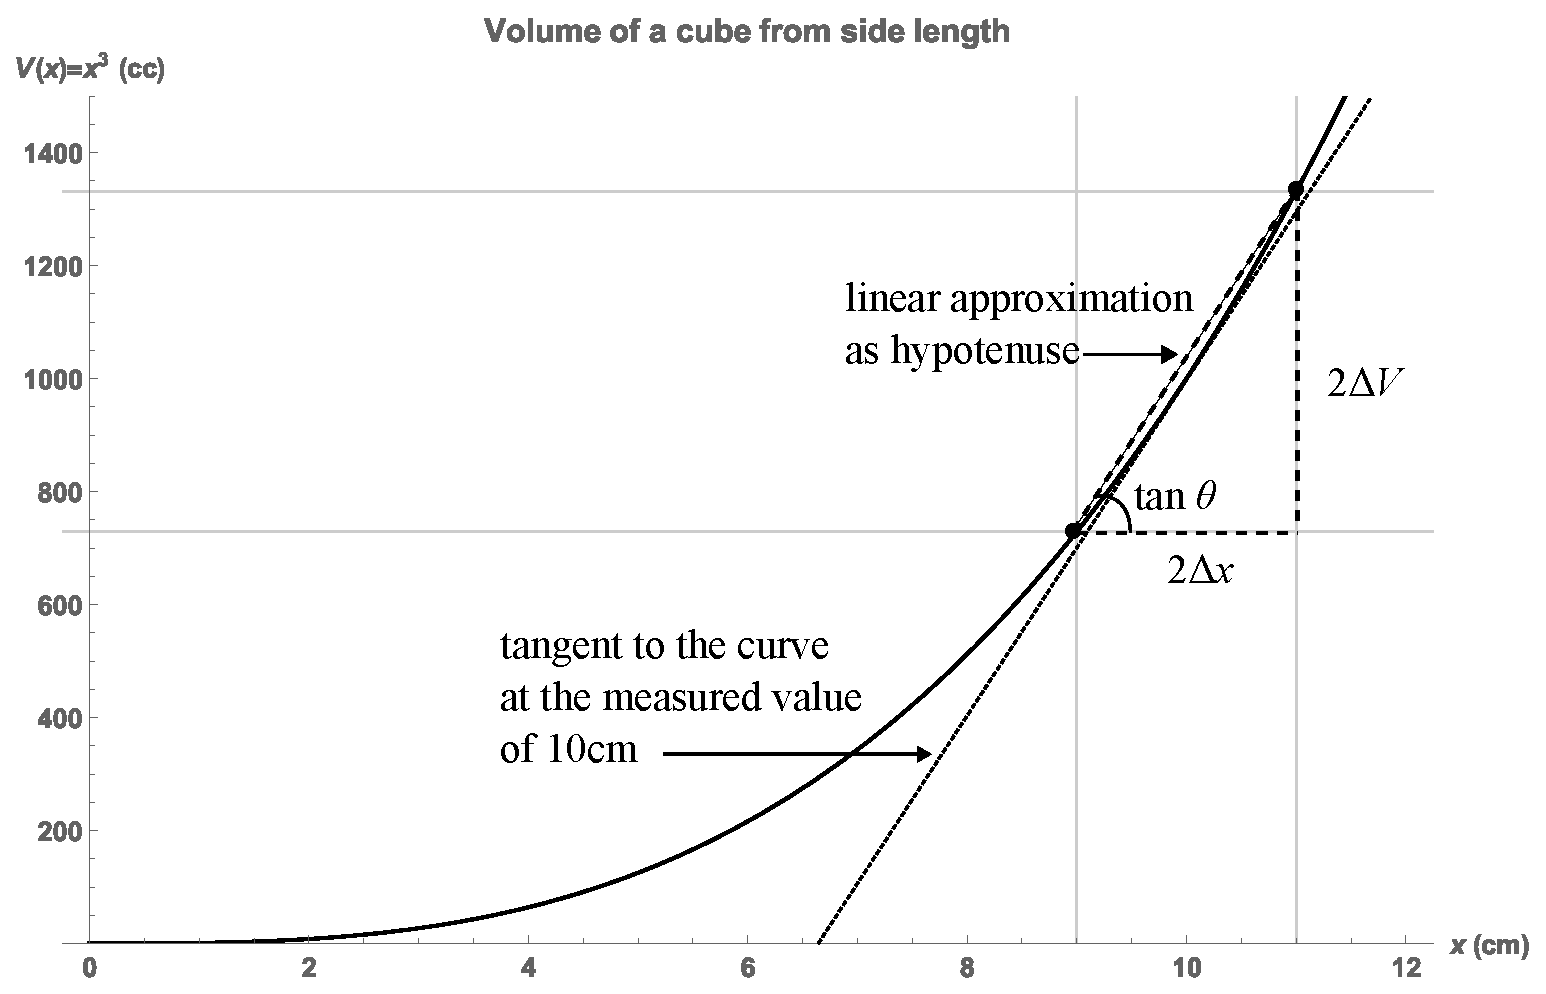
\includegraphics[scale=0.5]{0_intro/cubing.eps}
\caption{Error propagation through cubing a length.}
\label{fig:intro:cubing}
\end{figure}

We can illustrate the situation graphically, as in fig. \ref{fig:intro:cubing}.
The length measured varies from 9 to 11 cm, the interval bounded by
the vertical lines. The corresponding volume varies from $9^{3}=729$cc
and $11^{3}$=1331cc, the interval between the horizontal lines. That
is, a length uncertainty of 11-9=2cm gives rise to a volume uncertainty
of 1331-729=602cc. Now, only half of the width of the uncertainty
is denoted by $\Delta x$ and $\Delta V$, since the error lies on
either side of the base value as a $\pm$. (This is why the horizontal
and vertical lengths in the plot that correspond to the uncertainties
are $2\Delta x$ and $2\Delta V$ respectively.) So a $\Delta x=1$cm
gives rise to a $\Delta V=301$cc. Quite a lot, since the cubed function
amplifies its argument, and hence differences in its arguments as
well.

Here we have explicitly calculated the propagated error in the volume
by applying the function to the two extreme values of the erroneous
original quantity, taking the difference and halving it. But there's
a shorter way to do this.

Consider the rectangular region in the plot bounded by the error boundaries.
We can approximate the curve in that region to be a straight line
segment with slope equal to the slope of the curve at that point,
given by $\frac{\partial V}{\partial x}$ at $x=10$cm. Then we consider
the triangle created by the horizontal error, the vertical error,
and the hypotenuse which is that straight line, and this gives us
a simple relation between the base and perpendicular:

\begin{equation}
\frac{2\Delta V}{2\Delta x}=\tan\theta=\frac{\partial V}{\partial x}\Rightarrow\Delta V(x)=\frac{\partial V}{\partial x}\Delta x.
\end{equation}


Using this relation, what do we get as the propagated error in volume?
We get:

\begin{equation}
\Delta V(x)=\frac{\partial V}{\partial x}\Delta x=3x^{2}\Delta x=3\times\left(10\textrm{cm}\right)^{2}\times1\textrm{cm}=300\textrm{cc}.
\end{equation}


This is \textit{not} the same as the actual propagated error of 301cc
that we explicitly calculated!

The reason is the linear approximation we made. However, in practical
situations when the error is not too big so that the function may
be considered linear in the small error region, this provides a good
approximation, as it did now.

You will notice that this simple derivation hasn't given us the absolute
sign of eq. \ref{equ:diff:single-uncertainty}. To understand the necessity of the absolute sign,
note that the partial derivative may be negative depending on the
function, but an error is always positive. A more detailed justification
will follow later.

We now consider a physical way to extend this to multiple variables,
that gives rise to eq. \ref{equ:diff:uncertainty}.

Suppose you know the temperature at every point of a room, as a function
$T(x,y,z)$ where $x$, $y$ and $z$ are the coordinates used to
mark points in the room. Someone asks you what the temperature is
at a point. You locate the point by measuring out its coordinates
with a ruler. This will have uncertainties, so that the coordinates
of the point are $(x\pm\Delta x,y\pm\Delta y,z\pm\Delta z)$. Since
you don't have the location exactly pinpointed, the temperature you
report shall also have an uncertainty $\Delta T$ owing to this variability.
What is this uncertainty?

\begin{figure}[!htb]
\centering
\epsfxsize=12cm 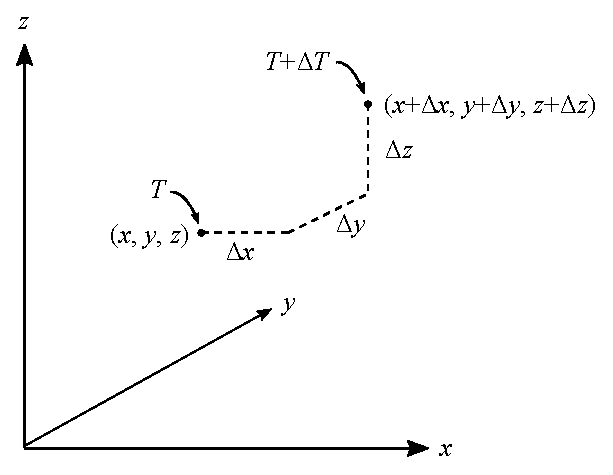
\includegraphics{0_intro/temperature.eps}
\caption{Temperature variation in a room (example of error propagation for a multi-variable function).}
\label{fig:intro:temperature}
\end{figure}

Consider going from the point $(x,y,z)$ where the temperature is
$T$ to the point $(x+\Delta x,y+\Delta y,z+\Delta z)$ where the
temperature is $T+\Delta T$. One way to go about this is to first
move by $\Delta x$ along the $x$-axis. According to simple calculus,
the change in temperature due to this is the rate of change of temperature
with respect to change in $x$, multiplied by the increment in $x$,
i.e. $\frac{\partial T}{\partial x}\Delta x$. It is a partial derivative
because we are changing only one variable and holding the other variables
fixed. Similarly, the contributions to the change of temperature due
to moving along the other two axes are $\frac{\partial T}{\partial y}\Delta y$
and $\frac{\partial T}{\partial z}\Delta z$. This completes our move,
and the total change of temperature has been:

\begin{equation}
\Delta T=\frac{\partial T}{\partial x}\Delta x+\frac{\partial T}{\partial y}\Delta y+\frac{\partial T}{\partial z}\Delta z.
\label{equ:intro:temperature}
\end{equation}


\textbf{A crucial point to note} in this derivation is that the arguments of
the function must be \textit{independent} variables, so that it is
possible to vary one of them while keeping the other ones fixed. This
means that when we consider the error of a multi-variable function,
we should identify the correct independent variables that it is a
function of. For example, if our function is $x^{2}+xy$, then we
cannot see it as a function of $x^{2}$ and $xy$ and write its error
in terms of partial derivatives with respect to those, because we
cannot independently vary either of those variables without changing
the other.

Once again, note that we have not derived the absolute sign of \ref{equ:diff:uncertainty} in our
simple explanation. We shall now give a bit more detailed justification
for the absolute sign in the general case of a multi-variable function.

We consider a two variable example. Suppose someone has asked you
to find the difference of two lengths. You measure the lengths to
be $x\pm\Delta x=50\pm5$cm, i.e. it can be between 45 and 55cm, and
$y\pm\Delta y=10\pm1$cm, i.e. between 9 and 11cm. The difference
function is $f(x,y)=x-y$. The base value of the difference is of
course 50-10=40cm, but what is its error?

If we naively use eq. \ref{equ:intro:temperature} without the absolute signs, then we shall
get:

\begin{equation}
\Delta f(x,y)=\frac{\partial f}{\partial x}\Delta x+\frac{\partial f}{\partial y}\Delta y=\Delta x-\Delta y=4\textrm{cm}.
\end{equation}


However, is this true? The largest possible value of the difference
is when the first length is the greatest (55cm) and the second is
the least (9cm), which gives us 55-9=46cm. The smallest value of the
difference comes from the smallest value of $x$ (45cm) and the largest
value of $y$ (11cm), yielding 45-11=34cm. Thus, the variation of
the difference is between 34 to 46cm, an uncertainty of 12cm. Half
of this is $\Delta f(x,y)$, which is then 6cm.

This corresponds to $\Delta x+\Delta y$, not $\Delta x-\Delta y$.
Why did this happen? Well, even though we are subtracting the two
lengths, we cannot be sure that their errors will also subtract. We
could have made a positive error in one length and a negative error
in the other, in which case they would end up adding together in the
same direction even though we are subtracting the lengths. Thus, the
unknown sign of the individual errors could conspire together to add
in the worst case scenario. The uncertainty of the propagated value
corresponds to the most general, worst case scenario, and therefore
we should always add the absolute errors contributed by the variability
of each of its arguments. This explains the absolute signs in eq. \ref{equ:diff:uncertainty}.
Now that we have given a physical explanation for the single- and multi-variable error propagation formul\ae, we visit some examples that should make things clearer.
\vspace*{.5cm}  \\

\noindent {\bf Example:}  {\bf Addition and Subtraction} \\
Given: $f(x,y) = 3x+y-z+5$ \\
Find:  $\Delta f$ \\
\begin{eqnarray*}
\Delta  f & = & \left| \frac{\partial f}{\partial x} \right| \Delta x +
           \left| \frac{\partial f}{\partial y} \right| \Delta y +
            \left| \frac{\partial f}{\partial z} \right| \Delta z \\
 & = & \left|3 \right| \Delta x +  \left| 1  \right| \Delta y +\left|-1\right| \Delta z \\  
 & = & 3 \Delta x + \Delta y + \Delta z
\end{eqnarray*}
\noindent
{\bf Example:}  {\bf Multiplication and Division} \\
Given: $f(x,y) = x^2y/(5z)$ \\
Find:  $\Delta f$ \\
\begin{eqnarray*}
\Delta  f & = & \left| \frac{\partial f}{\partial x} \right| \Delta x +
           \left| \frac{\partial f}{\partial y} \right| \Delta y +
            \left| \frac{\partial f}{\partial z} \right| \Delta z \\
& = & \left|2 x y/ (5z)\right| \Delta x +  \left| x^2/(5z) \right| \Delta y +
\left|-x^2y/(5z^2)\right| \Delta z 
\end{eqnarray*}
\noindent  {\bf Example:}  {\bf Ohm's Law}\\
Given: $V = IR $ \\
Find:  $\Delta R$ \\
 \begin{eqnarray*}
\Delta R  & = & \left| \frac{\partial R}{\partial V} \right| \Delta V +
           \left| \frac{\partial R}{\partial I} \right| \Delta I \\
  & = & \left| \frac{1}{I} \right| \Delta(V) + \left| \frac{-V}{I^2} \right| \Delta I
\end{eqnarray*}

\subsection{Agreement within uncertainty} %neel
\label{sec:intro:agreement}
A very important idea in the sciences and engineering is to decide when two quantities agree with each other. This could be values for a quantity measured or calculated independently by different people or research groups, or by the same person but using different methods.

If the quantity has no error, such as the number of tentacles of a newly discovered marine species, the question of agreement is simply to check if the number is the same.

But if the different observations of the quantity come with errors, they need to {\it agree within uncertainty}. The following explains how this is done, and you will need to use this in several places throughout this course.

Suppose we have two measurements $x_1 \pm \Delta x_1$ and $x_2 \pm \Delta x_2$ of the same quantity. Then we essentially need to check if their regions of uncertainty overlap. If they do, the quantities have a common overlap region and they agree within uncertainty, otherwise not.

If you consider fig. REF, you will see that this implies simply to check whether the distance between the base values is greater or less than the sum of their uncertainties, i.e.:

\begin{center}
$\left|x_1-x_2\right| \stackrel{?}{\gtrless} \Delta x_1 + \Delta x_2$
\end{center}

If it is greater, the quantities don't agree, and if it is less, they do agree. If it is exactly equal, it would also be considered agreement because the value on the boundary is common.

\subsection{Reporting Erroneous Quantities} %neel
\label{sec:intro:reporting}
Now that we have a clear idea of  what constitutes  the uncertainty of a 
measurement, how to estimate it, and how to propagate it, we should talk about
the proper way to report the uncertainty of a quantity. The following instructions explain the format of reporting quantities with errors. We take as an example a mass measurement of 14,877 g (we call this the base value) with an error of .5 kg. 
\begin{enumerate}
\item Convert the base and error to decimal expressions.

\item Convert both the base value and the error to the same unit and order. In our case, if we choose everything to be in kg, we convert the base value to 14.877 kg.

\item Either round off or add zeros to the base value so that it is up to the same decimal place as the error.

In our case, therefore, the base value is rounded to 14.9 kg. If the error had been .5021 kg, the base value would have become 14.8700 kg.

Thus, the error takes priority. This is easy to understand: it is the error that determines the amount of information. If we have fewer decimal places in the error than the base, then we don't really know the base up to its last place, do we? So we must round off to the last place of the error. And if the error has extra decimal places, that means we have additional accuracy to add significant zeros to the base value.
\item Write down the base value `$\pm$'  the error, {\it followed by} the common order and the unit at the end. Don't put them next to both the base value and the error; this makes it look uglier, and harder to compare the base with the error immediately. This is not a hard rule though, nevertheless the best practise.
\end{enumerate}

In summary, the correct way to report an erroneous quantity is:

\begin{center}
$14.9 \pm 0.5$ kg or $(14.9 \pm 0.5) \cdot 10^3$ g etc.
\end{center}

The following are some wrong ways, with explanations of what mistakes have been made.
\begin{itemize}

\item Quantities have not been converted to decimal:
\begin{center}
$\pi \pm \frac{2\pi}{3}$ rad or $\sqrt{2} \pm \frac{1}{3}$ Hz.
\end{center}
Expressions like $\pi$, $e$, $\sqrt{2}$ etc and recurring fractions like $\frac{1}{3}$ imply {\it infinite} digits, and it is of course impossible that that's how much accuracy you have.

\item Different units for base and error:
\begin{center}
$14.9$ kg $\pm 1.1$ lb.
\end{center}

\item Different orders for base and error (this is a common error!):
\begin{center}
$14.9$ kg $\pm 0.5 \cdot 10^3$ g or $20.2$ km $\pm 300$ m or $3 \cdot 10^9 \pm 2 \cdot 10^7$ V.
\end{center}


\item Base and error have not been rounded to the same place (also very common!):
\begin{center}
$14.877 \pm 0.5$ kg or $14.877 \pm 0.5021$ kg.
\end{center}

\item Order and unit have been repeated:
\begin{center}
$14.9 \cdot 10^3$ g $\pm 0.5 \cdot 10^3$ g.
\end{center}


\end{itemize}

These are the rules you will use most often in reporting your results. They 
become rather cumbersome, though, when you begin to make very precise 
measurements. Consider, for example, the charge on the electron; the best 
measurement we have of this number is
\begin{eqnarray*}
(1.60217733 \pm 0.00000049) \cdot 10^{-19}~{\rm C}.
\end{eqnarray*}
Writing so many zeroes and taking care of the aligning is very annoying; so, we've developed a shorthand for reporting these 
kinds of measurements. You simply quote the result to the known uncertainty and
place the uncertainty of the last few digits in parentheses after the number 
and before the power of ten. In this notation, the electron's charge is
\begin{eqnarray*}
1.60217733(49) \cdot 10^{-19}~{\rm C},
\end{eqnarray*}
which is much easier to deal with. This notation also provides a natural way to adhere to the rules of representation and makes it harder to make mistakes in the format, so you're recommended to use it.

Finally, in various experiments we quote what are called ``accepted values''
for various physical parameters. These are the scientific community's best 
estimates of these numbers. They have been experimentally verified and checked 
for consistency with other measurements. Most you will find are very precise, 
typically 6 or 7 decimal places. You will discover in trying to do your own 
labs that making such high precision measurements is not easy. They also let 
you know that there is still some uncertainty in these parameters; they are
not {\em exact}; but you will probably not be able to help narrow that using 
the equipment and techniques we have, which means they are exact as far as we 
can tell. So, keep in mind as you attempt to verify these numbers, that other 
folks had to do these measurements too.  

\section{The Lab Worksheet}

The lab worksheets are preformated to be well organized, concise, and 
complete.  The worksheets are designed to maximize
your efficiency.  The format of the worksheets includes the following:
\begin{itemize}
\item  In-Lab Procedure \\
\item  In-Lab Computer Work \\
\item  Pre-Classroom Checklist \\
\item  In-Classroom Calculations \& Analysis \\
\item  In-Classroom Discussion  and Conclusion \\
\end{itemize}
Each item is described in detail below.  Some may occur more than once in any 
given worksheet.

\subsection{In-Lab Procedure}

The In-Lab Procedure section will guide you through experimental
set-up, data collection, and necessary calculations.  This section
will always be the first section of the worksheet, but there may be a
few of them in any one worksheet.  Each time you set-up a new
experiment in that day's lab, a new in-lab procedure section will
guide you.  Since this lab is electronics and optics, you will be
connecting circuits and manipulating optical equipment.  Figures are
provided and numbered to show you how to make connections and
placements for these set-ups.  The figures will become your friends in
setting up the experiments.  {\bf Do not ignore them}.  You cannot set-
up without the figures.  
 
After setting up the experiment, you will follow the directions given
to begin data collecting.  Sometimes you will be obtaining one piece
of data, other times twenty.  Any data collecting will be specified
and organized by a table or space.  Blank spaces above answers are to
be used by you to {\bf show your work} in reaching the answer below
the space.  This is {\bf very important} as indicated by the {\bf
boldface}.  Boldface will appear when an important point is being made
vital to your grade.  

When you are recording your data, be that in a table or
on a line, you should present your raw data neatly and completely
including {\bf units}, uncertainties, and significant digits.  Any
calculations used in recording the data should be shown in the space
provided above the answer.  Show all calculations {\it keeping numbers
out of the calculations until the final step}.  How to do the
calculations will be explained in the In-Classroom Calculations \&
Analysis section. 

When showing your work, it is crucial that you {\it propagate} all units 
and uncertainties through the algebra. This will convince the reader
that you're not trying to hide anything and it will help you check
your answers as you go.  Do not ignore units for several steps of a
computation and then just write down what seems to be the proper
units; you can loose many factors of 10 by not doing this. 

Before moving on to the next section of the worksheet, 
double check that you have completed everything required of you.  
Remember that this section is not only for data recording.  Just because 
there is no space for an answer does not mean there was nothing important
to be done.  You must complete everything in each section before moving on
to the next one.  You and your lab partner can divide the work to be more
efficient but make sure you do everything. 

\subsection{In-Lab Computer Work} 
After collecting and recording data you will usually make a graph.
You are not plotting the data to make more work for yourselves.  The
graphs will give you a vital piece of information that you will use in 
calculations,
analysis, discussion or conclusion.  Graphing is usually the easiest
and most accurate way to get the information.  You will be using the computers
in lab, and that means that you must complete all the graphs in the two hour
lab time.  You will need them for the classroom period.   

KaleidaGraph is the plotting program you will be using for all 
your graphs.  You will spend part of the first two lab sections
learning and practicing your KaleidaGraph skills.  You need to become 
proficient in KaleidaGraph to complete the labs   
since you will include all graphs with your worksheet before leaving lab.
You should title your graphs appropriately, include
all units, and label axes.  Despite the fact that the computer will be
doing most of the work in graphing your data, you need to understand
what the work entails.  

In many labs you will have to graph sets of 5 to 15 data points 
and make 
linear fits to the data. If you graph by hand, as you will in 
$\S$~\ref{sec:ea:graph}, you should use graph paper of at least 4 boxes per 
inch and each graph should be large and clear. A full
page graph of 10 points is not unreasonable. The scales on the axes should be 
appropriate for the data ranges, so that the data covers most of the graph. 
Having bunched up data points leads to difficulty in reading the graph and 
loss of precision in fitting lines and calculating slopes and intercepts. Do 
not draw your axes across a full page and choose your scale in such a way that 
the data points occupy only a few cm$^2$! Also, take care to distinguish 
dependent and independent variables when graphing; the quantity which is the 
function of the other in the experiment is conventionally plotted along the 
vertical axis. If you are asked to plot $y$ vs. $x$, for example, you should 
interpret $y$ as the dependent variable and plot it on the vertical axis. 
Always label the axes with their appropriate physical parameters and include 
the correct units in the label.

When fitting data by hand, as opposed to the least squares method discussed 
earlier, be sure not to obscure any data points and do not ``connect the 
dots.'' Doing so has no physical basis and yields no insight into the physics 
at hand. Using a straight edge, ``eyeball'' the line that best fits the data.
This line will yield the best values for the slope and intercept of your fit.
Furthermore, you should draw the steepest and shallowest lines that 
are consistent with both the trend of your data and with the error bars. 
These lines will yield the uncertainty in your fit parameters, through the
formulae
\begin{eqnarray*}
\Delta a &=& \frac{|a_{\mbox{steep}}-a_{\mbox{shallow}}|}{2} \\
\Delta b &=& \frac{|b_{\mbox{steep}}-b_{\mbox{shallow}}|}{2}.
\end{eqnarray*}
Remember that these lines represent the trend present in your data and might 
not pass through any data points. When calculating slopes for these lines, you 
want to choose two points on the lines that are not data points. The trend of 
the line is far more important than the slope between any two data points. 

Although these instructions tell how to estimate the best fit line by hand, the
computer is only doing a more sophisticated and reproducible version of this; 
thus, to fully employ the computer's power, you need to understand how to 
estimate these things independently of the computer. This will also help you 
check the results the computer gives you.

\subsection{Pre-Classroom Checklist}
The checklist is included for you to use as a check against what you have
to take out of the lab period.  You only have 2 hours in lab during which
time you may do several procedures and graphs.  Before leaving the laboratory, 
you will use this list to see that you have completed everything and have it
with you to take to the classroom.  Once you leave the lab, another class
enters it so you can't go back to use the computers or redo a portion of the 
lab.  The worksheet has been designed to be completed in parts.  You
will complete one procedure and do its computer work before moving on to 
the next procedure.  In this manner, you will be able to do a complete
analysis and discussion on at least some parts even if you don't finish
the lab.  

There are $\bigcirc$ provided for you to physically check off.  Do this.
It will keep you organized when you get to the classroom.  One hour
is not a lot of time to finish all the calculations, discussions, and 
conclusion.  Also make sure that each partner has her/his own data,
graphs, tracings, etc..  Contact amongst you will be kept to a minimum.


\subsection{In-Classroom Calculations \& Analysis}
At this point you have finished all In-Lab Procedures and In-Lab 
Computer Work.  You have also checked all the circles in the
{\bf check list} to ensure that you have completed all the laboratory
work.  Once the two hour lab period is over, you will move to the
classroom and finish the worksheet in {\bf one hour}.  If you
complete all in-lab sections sooner than two hours you may begin
the in-classroom sections.  

The calculations you need to do are clearly stated with referenced
equations, figures, and tables when appropriate.  There is a line
or space left for each answer.  There is also room for you to 
{\bf show your work}.  You must show all the steps and reasoning behind
your answers to get full credit.  A sample calculation is done for you
here as a future guide.  Suppose the question in the in-classroom 
calculation \& analysis section reads: \\
\vspace*{0.3cm}  \\
\noindent \hspace*{1cm} Calculate the resistance through a circuit given the 
voltage, $V$ = \\
\hspace*{1.2cm}5.00 $\pm$ 0.01 $V$, and current, $I$ = 20.0 $\pm$ 0.2 $mA$, 
with uncertainties \\
\hspace*{1.2cm}and units.  {\bf Show Work}. \\
\begin{eqnarray*}
V & = & IR \\
R & = &  \frac{V}{I}  \\
R  & = &  \frac{5 \> V}{20\>mA} \\ 
R  & = &  250\> \Omega \\
\Delta R  & = & \left| \frac{1}{I} \right| \Delta(V) + \left| \frac{-V}{I^2} \right| \Delta I\\
\Delta R   & = & \left| \frac{1}{20 \> mA} \right| 0.01 \> V + \left| \frac{-5 \> V}{400 \> (mA)^2} \right| 0.2 \> mA \\
\Delta R  & = &  3 \> \Omega \\
R  & = & 250 \pm 3 \> \Omega 
\end{eqnarray*}
\noindent The above is what you should show and report.  Note that
numbers were not used until the last line of each calculation and
the uncertainties were treated separately from the values.  You will
be performing this calculation later in lab.  

The In-Classroom Calculation \& Analysis sections can also
ask questions that lead you to an understanding of the reasoning behind
the lab and the physical principles that the lab confirms.  They are rarely
in yes/no format.  Answer all the questions completely, stating
your reasoning leading to the answer and showing any calculations or
drawings necessary.  At the end of this section you should understand
all aspects of the lab well enough to write a concluding statement.

\subsection{In-Classroom Discussion and Conclusion}
In the final section you will bring all your analysis 
together to answer questions and make 
specific, concrete conclusions about the parameters and physics developed in 
the lab. This includes a clear statement of the results of the lab, 
{\it e.g.}~parameters that you've measured including units and uncertainty, 
comments on the physical implications of these parameters, etc. You should 
indicate whether your results are consistent with previous efforts and discuss 
the internal consistency of your experiment. You should candidly address the 
uncertainties that arose in the lab and attempt to unambiguously and uniquely 
identify the key source of error. Within the paradigm that we discussed before,
this cannot include things like ``human error'' or ``errors in the 
calculations.'' You should have these illegitimate errors tightly under 
control. With all these ideas clearly laid out, you should then state whether 
you believe the experiment to be a success or not, justifying yourself by 
referring to your previous discussions.

Your instructor may also assign additional questions for you to ponder. You 
should incorporate the answers to these questions into your discussion.

\vfill
\pagebreak

\renewcommand{\thesection}{\thechapter.W1}

\section{Using KaleidaGraph for Data Analysis} %neel
\label{sec:hypoexp}
\subsection{A Hypothetical Experiment}

The software package known as KaleidaGraph can be a useful tool for
data analysis. In this section you shall plot and fit data collected from an imagined experiment to familiarize yourself with the software.

A version of Murphy's law states that if a piece of buttered toast falls on an expensive carpet, the more butter you put on it, the less likely that it would have fallen butter-side up. This assertion can be represented by an equation:

$$P = a{1 \over V}, $$ where $P$ represents the probability of a piece
of toast falling butter-side up, $a$ is a proportionality constant,
and $V$ is the volume of butter applied on the toast.

Thus, if you collected measurements of these over several trials, and plot $P$ against ${1 \over V}$, you'd expect the points to lie roughly along a straight line through the origin, with a slope equal to $a$. This is what you shall verify.

Suppose an experiment has been performed that tests this. Various amounts of butter were applied to toast, and dropped many times on a carpet. The fraction of times it fell butter-side up was expressed as a probability. The results of the experiment are:
\begin{center}
\begin{tabular}{|c|c|}
\hline
$V$(cc) & $P$ \\ $1.0 \pm 0.1$ & $0.43 \pm 0.01$ \\ $2.5 \pm 0.6$ & $0.15
\pm 0.01$ \\ $5.0 \pm 0.2$ & $0.09 \pm 0.01$ \\ $7.5 \pm 0.2$ & $0.06 \pm
0.01$ \\ $10.0 \pm 0.3$ & $0.04 \pm 0.01$ \\
\hline
\end{tabular}
\end{center}  


\subsection {Entering Data}
KaleidaGraph holds data in a {\bf data window.} One of these should
appear when you start; its default name is {\bf Data 1.} Enter all the data here, entering values for $V$ in column ``A'',
the uncertainties $\Delta V$ in column ``B'', the values for $P$ in column ``C'' 
and the uncertainties $\Delta P$ in column ``D''.


\subsubsection{Renaming Columns of Data}

KaleidaGraph labels the axes on plots with the name of the columns it used in the plot. The default names of columns are ``A'', ``B'', ``C'', etc. These appear in
the {\bf column title} row of the data window, along with a number. To
change the name of the column,

\noindent
\begin{enumerate}
\item Double-click on the column title you wish to change.
\item In the ``Column Format:" dialog box which appears there will be a list of column 
titles. Highlight the title you wish to alter by clicking on it.
\item Type in the new title of the column (for example ``A'' becomes $V$(cc)). Don't forget units in parentheses for any columns. Click {\bf Done.}
\end{enumerate}

The number of any column can be set to zero merely by clicking on the
title cell of that column. The columns to the right then take the
numbers 1, 2, 3... The columns to the left become unnumbered.

\subsection{Entering Formulas}

Often, the raw data you enter is not immediately in the form you need
for plotting. KaleidaGraph is capable of performing
mathematical operations on the numbers you have entered. One way of
using this feature is to define a formula for KaleidaGraph. Formulas
tell KaleidaGraph to put in one column the result of operations on
data in other columns.

The syntax of formulas you define should be
\begin{center}
c$x$ = f(c$y$, c$z$, ...)
\end{center}
where $x, y,$ and $z$ are the numbers of the columns which contain the
numbers you wish to operate on, and f(...) is the mathematical
expression you wish KaleidaGraph to calculate.

For example, since you want to plot $P$ vs. $1/V$,
you need to make a column containing
the the $1/V$ values. For this,

\noindent
\begin{enumerate}
\item From the {\bf Windows} menu at the top of the screen, select the option {\it
Formula Entry.}
\item In the ``Formula Entry'' window which appears, click on one of the buttons 
labeled {\bf F1 - F8.}
\item Type in the formula in the space provided in the ``Formula Entry'' window (in your case, c4 = 1/c0).
\item Click the button marked Run in the ``Formula Entry'' window.
\end{enumerate}
\indent

The button labeled {\bf F1-F8} you choose corresponds to one of the
function keys at the top of the keyboard. Pressing that key will bring
up the ``Formula Entry'' window again, this time containing the
formula you defined {\bf thus saving important formulas for you}. Make 
sure to rename the column you just made.

Of course, the uncertainties in $1/V$ are different from the
uncertainties in $V.$ So you'll need to get KaleidaGraph to calculate
an uncertainty column for you. Figure out the necessary formula.

\subsection{Plotting Data}

\subsubsection{Making a Scatter Plot}

\noindent
\begin{enumerate}
\item Activate the window containing the data you want to plot by clicking on it.
\item From the {\bf Gallery} menu at the top of the screen, select the {\bf Linear}
submenu, and from that select the {\bf Scatter} option.
\item A dialog box will appear. In it, there will be columns of circles labeled ``X"
and ``Y." Under ``X" click on the circle in the row containing the
title of the column which contains the x-coordinates of your data. A
solid black circle should appear.
\item Do the same with your y-coordinates in the column labeled ``Y."
\item Click on the button labeled {\bf New Plot.}
\end{enumerate}
\indent

\subsubsection{Adding Error Bars}

\noindent
\begin{enumerate}
\item Activate the window containing your plot by clicking on it.
\item From the {\bf Plot} menu at the top of the screen, select the option ``Error
bars..."
\item In the ``Error Bar Variables" dialog box which appears, click on the square
labeled ``X Err.''
\item Click and hold on one of the two rectangles labeled ``\% of values," and select
the option ``Data Column."
\item Select the column which contains the uncertainties in the x-coordinates of your
plotted data.
\item Now, follow the same procedure starting with the square labeled ``Y Err.''
\item Click on button labeled {\bf Plot.}
\end{enumerate}
\indent

\subsubsection{Writing a good graph title}%neel
A good, descriptive title for plots is essential in engineering and the sciences to convey what the plot is about. Here are some pointers about writing the title.
\begin{itemize}
\item Don't leave your graph title as the default `Data 1' and suchlike. This is not useful at all.
\item Don't also merely repeat the axis labels for the graph title, e.g. in this case, the title shouldn't just say `$P$ vs $1/V$' or even `Probability vs Inverse of butter volume'. An ideal graph should already provide detailed axis labels like `Probability of landing butter-side up $P$' and `Volume of applied butter $V$ (cc)', so that it is redundant to repeat them in the plot title.
\item Then what should be in the title? It should provide context, i.e. a description of where the data came from. In this case, a good title would be `Testing Murphy's law by dropping buttered toast.'
\item When thinking about the title, imagine slipping the printed plot under the door of any scientist in the building, who has no information otherwise of what that plot is. Will they understand what this plot is about? It is the job of the title to give the rest of the information context and meaning in a condensed description.
\end{itemize}
Always keep these pointers in mind while naming plots throughout the rest of this course.

\subsection{Performing a Weighted Least-Squares Fit}
Now we shall obtain the slope and y-intercept of the best fit line through the data, by means of an error-weighted least-squares fit.
\noindent
\begin{enumerate}
\item Activate the window containing your plot by clicking on it.
\item From the {\bf Curve Fit} Menu at the top of the screen, select the {\bf General}
submenu, and from that, select the option {\bf fit1.}
\item In the ``Curve Fit Selections:" dialog box which appears, click on the button
labeled {\bf Define...}
\item In the new dialog box that appears, click on the square labeled ``Weight Data"
so that an X appears in it.
\item Click on the button labeled {\bf OK.}
\item In the ``Curve Fit Selections:" dialog box, click on the square next to the
column title which contains the error in the
y-coordinate of the data you are
plotting.
\item A new dialog box will appear called ``Weight Data From Column:". By clicking on
the buttons labeled $\ll$ and $\gg$ , make sure the name of the
column containing the uncertainties for the y-coordinate appears in
the window.
\end{enumerate}
\indent

Now you need the numerical results of the fit. Simply choose the
``Display Equations" option from the {\bf Plot} menu, and a table
containing the numbers you desire will appear. Note that, in this
table, m1 is the y-intercept and m2 is the slope of the best fit line.

\subsubsection{The Work You Should Turn In}

Attach the plot printout to the worksheet that follows. This printout 
should contain: properly labeled axes and plot title, x and y error bars, best fit line, and the box of calculated parameters from the line.\\
{\bf Below the plot, report in a complete
sentence what you have found to be the constant of proportionality from the fit
(with uncertainty).} \\



\vfill
\pagebreak
%$$
%$$
%\vfill
%\clearpage
%\newpage

%  Label worksheets by \thechapter.W1
\renewcommand{\thesection}{\thechapter.W1}

\section{In-Classroom Calculations}
{\bf \Large Name:}~ \rule{5cm}{.1mm}~~~~~~~
{\bf \Large Day/Time:}~\rule{3cm}{.1mm}\\

\noindent
{\bf Instructions}: Perform all of the following 
calculations using the techniques explained in 
Chapter~0 (Introduction) of the lab manual. Show all calculations explicitly, 
propagate uncertainties where appropriate, include the proper number of 
significant figures, and provide units. 

\subsection{In-Lab Procedure}

Perform the KaleidaGraph practice plot and analysis in the previous
section $\S$~\ref{sec:hypoexp} and attach it the end of this worksheet.

\subsection{In-Classroom Calculations}

\begin{enumerate}

\item Four independent measurements 
of the voltage supplied by 
a certain D-cell battery were made:
\vspace*{-5mm}
\begin{center}
\begin{tabular}{c}
$2.4\pm 0.6$~\mbox{V} \\
$2.96\pm 0.08$~\mbox{V} \\ 
$3.02\pm 0.06$~\mbox{V} \\ 
$2.968\pm 0.004$~\mbox{V}.
\end{tabular}
\end{center}
\vspace*{-3mm}
Referring to $\S$~\ref{sec:intro:uncert}, calculate the {\it most probable value}  of the D-cell voltage as well as the
standard deviation of the measurements using equations (\ref{eq:intro:average})
and (\ref{eq:intro:standdev}).  Write your answer as you would report the
final result. \\
\vspace*{5cm}\\

\pagebreak
\item Refer to $\S$~\ref{sec:intro:reprtun} for the calculation and 
propagation of uncertainty.
Two lengths have been measured to be $L_1 = 4.8 \pm 1.2$~cm 
and $L_2 = 3.2 \pm 1.6$~cm. 
\begin{enumerate}
\item Calculate the sum $L=L_1+L_2$ and its {\it absolute} uncertainty, 
$\Delta L$. \\
\vspace*{2cm} \\
\noindent Use these to calculate the {\it relative} uncertainty in $L$. \\
\vspace*{2cm} \\

\item Calculate the difference $L_0=L_1-L_2$, as well as its absolute and
relative uncertainties. \\
\vspace*{2cm} \\
\noindent Compare these uncertainties with those in the sum. \\
\vspace*{2cm} \\

\item Now calculate the product $P = L_1 L_2$ and its absolute and relative
uncertainties. \\
\vspace*{2cm} \\

\item Calculate the quotient $Q=L_1/L_2$, its absolute and relative
uncertainties. \\
\vspace*{2cm} \\
\noindent Compare the uncertainties to those in the product. \\
\vspace*{2cm} \\

\item Express $L$, $L_0$, $P$, and $Q$ in proper form, i.e. with units and 
uncertainties.  \\
\vspace*{3cm} \\
\end{enumerate}

\item The area of a square has been measured to be $A=50\pm 6$~cm$^2$. What is
the length of one side of the square?  \\
\vspace*{2cm} \\

\item Two resistors, with resistances $R_1=540\pm 54~\Omega$ and 
$R_2=860\pm 86~\Omega$, are connected in parallel. Calculate the equivalent 
resistance, $R_{\mbox{eq}}$, of the combination using the formula 
$$ \frac{1}{R_{\mbox{eq}}} = \frac{1}{R_1} + \frac{1}{R_2}.$$ \\
\vspace*{10cm} \\

\item For $\phi=60\pm 3^\circ$, calculate $\sin\phi$ and $\tan\phi$.
(Hint: convert the angle to radians.) \\
\vspace*{3cm} \\

\item Given that $L=20\pm 4$~cm and $y=8\pm 2$~cm in the triangle\\
\vspace*{2mm}\\
\hspace*{4cm} \epsfxsize=5cm 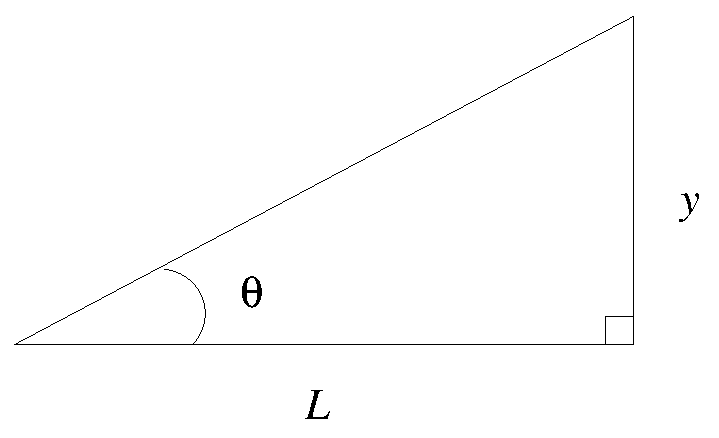
\includegraphics[scale=0.5]{0_intro/triangle.eps}\\
 %\epsfbox{intro_2/triangle.eps}
%\vspace*{2mm}\\
calculate $\sin\theta$. (Hint: it's not necessary to calculate the hypotenuse.)\\
\vspace*{3cm} \\
\end{enumerate}
\vfill
\noindent Attach your KaleidaGraph plot to the end of this worksheet. \\
{\Large Bring graph paper next week.} \\
{\Large End Error Analysis Worksheet}


\pagebreak
$$
$$
\vfill
\clearpage
\newpage

%  Label worksheets by \thechapter.W2
\renewcommand{\thesection}{\thechapter.W2}

\section{KaleidaGraph \& Graphing By Hand}
{\bf \Large Name:}~ \rule{5cm}{.1mm}~~~~~~~
{\bf \Large Day/Time:}~\rule{3cm}{.1mm}\\
\label{sec:ea:graph}
\subsection{In-Lab Computer Work}
\subsubsection{Two Exercises for Kaleidagraph}
\noindent
{\bf 1.} Imagine that you are riding in a car with your uncle Bob, his sister 
Sandy, and your cousins Rob and Gary. As you head down a back road in 
central Florida, a brilliant blue light suddenly bathes the car, and you
fall unconscious. When you wake up, you find yourself in a room with no 
doors and plain grey walls. An unknown source of illumination allows you
to see that your only company is a spark-tape apparatus, familiar to you
from your first semester lab class. You immediately realize that you can
conduct a simple experiment to determine the gravitational acceleration of 
the planet you are on. You conduct the experiment and find the following
distance fallen versus time data:

\vspace*{0.5cm}
\begin{center}
\begin{tabular}{|c|c|}
\hline
\multicolumn{2}{|c|}{Distance $(d)$ vs. time $(t)$ Measurements} \\
\hline\hline
$d$ (m) & $t$ (s) \\
\hline
  $.20 \pm .01$      &   $.2 \pm .02$   \\
\hline    
  $.80 \pm .04$      &   $.4 \pm .02$   \\
\hline
  $1.72 \pm .05$     &   $.6 \pm .02$   \\
\hline
  $3.16\pm .05$     &  $.8 \pm .02$    \\
\hline
  $4.84 \pm .10$     &  $ 1.0 \pm .02$    \\
\hline
  $6.96 \pm .10$      & $ 1.2 \pm .02$     \\
\hline
\end{tabular}
\end{center}

\vspace*{0.5cm}
\noindent
Do the following

{\it a)} Plot $d$ vs. $t^2$ and obtain a {\bf weighted} least squares fit.
(Remember, use {\bf fit1} under the General option of the curve fit menu.)
Error bars, properly labeled axes and units are essential!  All partners 
should have their own plots.  {\bf Show}
your work in finding $\Delta(t^2)$ below (only the error propagation formula, no numbers.) \\
\vspace*{2cm} \\

{\it b)} Determine the acceleration due to gravity from the results of 
your curve fit, including
units and uncertainties. Show work. \\
\vspace*{2cm} \\

\hspace{4cm}$g=$\rule{4.0cm}{.1mm}\\

{\it c)} Using the table of accelerations due to gravity of the planets that should be taped to the wall of the lab (or found online), guess where you are. (Hint: if you are high in the atmosphere, gravity will be reduced.) \\
\vspace*{0.8cm} \\

\noindent
{\bf 2.} In an experiment you will conduct in a few weeks, you will measure
the voltage $(V)$ of a discharging capacitor as a function of time $(t).$
You will be required
to plot 

$$
\ln \left( {V \over V_0} \right) \quad vs. \quad t
$$

\noindent
where $V_0$ is the initial voltage (that is, the voltage measured at time 
$t=0.)$

\noindent
Use the following sample data:


\vspace*{0.5cm}
\begin{center}
\begin{tabular}{|c|c|}
\hline
\multicolumn{2}{|c|}{Voltage $(V)$ vs. time $(t)$ Measurements} \\
\hline\hline
$V$ (V) & $t$ (ms) \\
\hline
  $4.0 \pm .10$      &   $ 0.0 \pm .02$   \\
\hline    
  $3.6 \pm .10$      &   $ 1.0 \pm .02$   \\
\hline
  $3.4 \pm .10$     &   $ 2.2 \pm .02$   \\
\hline
  $2.8 \pm .10$     &   $ 3.2 \pm .02$    \\
\hline
  $2.6 \pm .10$     &   $3.8 \pm .02$    \\
\hline
  $2.4 \pm .10$      & $5.0 \pm .02$     \\
\hline

\end{tabular}
\end{center}

\vspace*{0.5cm}
\noindent
Do the following

{\it a)} Plot $\ln (V / V_0)$ vs. $t$ and obtain a {\bf weighted} least
squares fit. Again, be sure to include error bars, units, and properly
labeled axes.  Remember, all partners must have their own plots.  
Show your work in finding $\Delta( \ln \frac{V}{V_0})$ (again, just the formula). \\
\vspace*{3cm} \\

{\it b)} Report the slope and intercept of your plot.
Units and uncertainties are a must! \\
\begin{table}[htb]
\begin{center}
\begin{tabular}{|c|c|}
\hline
Slope & Intercept \\
\hline
\hspace*{5cm} & \hspace*{5cm} \\
& \\
\hline
\end{tabular}
\end{center}
\caption{Slope and Intercept }
\end{table}

\subsection{In-Classroom Calculation \& Analysis}

\noindent This half of the worksheet is your only
practice in graphing by hand.  You will be using KaleidaGraph
to do all your graphing in Physics 103N.  Before using KaleidaGraph 
indiscriminately, first you will learn what graphing and least squares 
is all about.  Chapter~0 in the lab manual contains all the information
required to do this worksheet, refer back to the appropriate sections. \\

\noindent In Lab~2 (Electron Dynamics), we will learn that an electron 
moving in a 
constant electric potential~$V$ and a constant magnetic field~$B$ 
(perpendicular to the electron's motion), moves in a circular path of radius 
$R$, given by the formula
\begin{equation}
\fbox{$ \displaystyle R^2=\frac{2Vm}{eB^2}, $} \label{eq:1st:elect}
\end{equation}
where $m$ and $e$ are the mass and charge of the electron, respectively.\\

\subsubsection{Hand-fit Graphing}
\noindent A former group of 103N students set the magnetic field 
on their apparatus to
$B=1.154\pm 0.006$~mT (1~T = 1~Tesla = 1~kg/C~s) and measured the path radius
while varying the potential $V$:\\
\ \\
\begin{center}
\begin{tabular}{|c|c|}
\hline
$V$~(V) & $R$~(cm) \\
\hline %neel
$400\pm 20$ & $5.6\pm 0.4$ \\
$600\pm 20$ & $7.4\pm 0.4$ \\
$800\pm 20$ & $8.2\pm 0.4$ \\
$1000\pm 20$ & $9.0\pm 0.4$ \\
$1200\pm 20$ & $10.2\pm 0.4$ \\
\hline
\end{tabular}  
\end{center}

\begin{enumerate}

\item Plot $R^2$ versus $V$, including error bars on all points
on your graph paper.  Show your work in finding
$\Delta(R^2)$ in the space provided here. \\
\vspace*{2cm} \\
\noindent Does this look linear? \\
\vspace*{1cm} \\
\noindent Find the slope of the best 
line fit to the data. Use bounding lines to obtain the uncertainty in the 
slope.  {\bf Show all your work in the space provided below}. \\
\vspace*{8cm} \\

\subsubsection{Least Squares}
\item Now use linear least squares to obtain the slope with uncertainty. Note 
that $R^2$ is the {\it dependent} variable; you'll need to fill the following
table. Observe that there are two extra rows in it. Write the units of each column in the first row and the column sums in the last row. If you want you can use a spreadsheet program and either copy the results here or print it. %neel
\begin{center}
\begin{tabular}{|c|c|c|c|c|c|c|c|}
\hline
\multicolumn{8}{|c|}{Least Squares Method}\\
\hline 
  $V_i$ & $R_i^2$ & $\Delta (R_i^2)$ & $\frac{1}{(\Delta (R_i^2) )^2}$ &
$\frac{V_i}{(\Delta (R_i^2) )^2}$ & $\frac{R_i^2}{(\Delta (R_i^2) )^2}$ & 
$\frac{V_i^2}{(\Delta (R_i^2) )^2}$ & 
$\frac{V_i R_i^2}{(\Delta (R_i^2) )^2}$ \\
\hline
 & &  &  &  &  &  &  \\
\hline
 & &  &  &  &  &  &  \\
\hline
 & &  &  &  &  &  &  \\
\hline
 & &  &  &  &  &  &  \\
\hline
 & &  &  &  &  &  &  \\
\hline
 & &  &  &  &  &  &  \\
\hline
 & &  &  &  &  &  &  \\
\hline
\end{tabular}
\end{center} 

\noindent Now compute the sums required to find the slope, $a$, and
the uncertainty in slope, $\Delta a$, as in your lab manual. \\
\vfill
\pagebreak

\noindent Comment on whether the least squares result or the hand graph method is better by comparing their relative uncertainties. Do they agree within uncertainty (see § \ref{sec:intro:agreement})?  \\
%neel
\vspace*{4cm} \\

\item Use equation~(\ref{eq:1st:elect}) to calculate the charge-to-mass ratio
of the electron, $e/m$, from the value of $B$ and each of the slopes you obtained (hand fit and least squares), with uncertainty. Do they agree with the accepted value of $e/m=1.758~819~62(53)\cdot 10^{11}$ C/kg? § \ref{sec:intro:reporting} explains the parenthesis notation.\\ %neel

\end{enumerate}


\vfill
\noindent Attach your KaleidaGraph and hand plots to the end of this worksheet. \\
{\Large End Worksheet} 




% Go back to ordinary section numbering
\renewcommand{\thesection}{\thechapter.\arabic{section}}